\chapter{Overview}
\label{ch:detectors-overview}

% Intro shared by all subsections

\section{An International Physics Program}

The global neutrino physics community is developing a multi-decade
physics program to measure unknown parameters of the Standard Model of
particle physics and search for new phenomena.  The program will be carried out as an international,
leading-edge, dual-site experiment for neutrino science and proton decay studies, which 
is known as the Deep Underground Neutrino Experiment (DUNE).
The detectors for this experiment will be designed, built, commissioned and operated by the international DUNE Collaboration. The facility required to support this experiment, the Long-Baseline Neutrino Facility (LBNF), is hosted by Fermilab and its design and construction is organized as a DOE/Fermilab project incorporating international partners. Together LBNF and DUNE will comprise the world's highest-intensity neutrino beam at Fermilab, in Batavia, IL, a high-precision near detector on the Fermilab site, a massive liquid argon time-projection chamber (LArTPC) far detector installed deep underground at the Sanford Underground Research Facility (SURF) \SI{1300}{\km} away in Lead, SD, and all of the conventional and technical facilities necessary to support the beamline and detector systems. 


The strategy for executing the experimental program presented in this Conceptual 
Design Report (CDR) has been developed to meet the requirements 
set out in the P5 report~\cite{p5report} and takes into account the recommendations of the European Strategy for Particle Physics~\cite{ESPP-2012}. It adopts a model where U.S. and international funding agencies 
share costs on the DUNE detectors, and CERN and other participants provide in-kind contributions 
to the supporting infrastructure of LBNF. LBNF and DUNE will be tightly coordinated as DUNE collaborators 
design the detectors and infrastructure that will carry out the scientific program.
  
The scope of LBNF is
\begin{itemize}
\item an intense neutrino beam aimed at the far site
\item conventional facilities at both the near and far sites
\item cryogenics infrastructure to support the DUNE
  liquid argon time-projection chamber (LArTPC) detectors at SURF
\end{itemize}

The DUNE detectors include
\begin{itemize}
\item a high-performance neutrino detector and beamline monitoring system
located a few hundred meters downstream of the neutrino source
\item a massive LArTPC neutrino detector located deep underground at the far site
\end{itemize}

With the facilities provided by LBNF and the detectors provided by
DUNE, the DUNE Collaboration proposes to mount a focused attack on the
puzzle of neutrinos with broad sensitivity to neutrino oscillation
parameters in a single experiment.  The focus of the scientific
program is the determination of the neutrino mass hierarchy and the
explicit demonstration of leptonic CP violation, if it exists, by
precisely measuring differences between the oscillations of muon-type
neutrinos and antineutrinos into electron-type neutrinos
and antineutrinos, respectively. Siting the far detector deep underground will
provide exciting additional research opportunities in nucleon decay,
studies utilizing atmospheric neutrinos, and neutrino astrophysics,
including measurements of neutrinos from a core-collapse supernova
should such an event occur in our galaxy during the experiment's
lifetime.

%%%%%%%%%%%%%%%%%%%%%%%%%%%%%%%%%%%%%%%%%%%%%%%%%%%%%%%%%%%%%%%
\section{The LBNF/DUNE Conceptual Design Report Volumes}

%%%%%%%%%%%%%%%%%%%%%%%%%%%%%%%%%%%
\subsection{A Roadmap of the CDR}

The LBNF/DUNE CDR describes the proposed physics program and 
technical designs at the conceptual design stage.  At this stage, the design is
still undergoing development and the CDR therefore presents a \textit{reference design} 
for each element as well as \textit{alternative designs} that are under consideration.

The CDR is composed of four volumes and is supplemented by several annexes that 
provide details on the physics program and technical designs. The volumes are as follows

\begin{itemize}
\item \volintro{} provides an executive summary of and strategy for the experimental 
program and of the CDR as a whole.
\item \volphys{} outlines the scientific objectives and describes the physics studies that 
the DUNE Collaboration will undertake to address them.
\item \vollbnf{} describes the LBNF Project, which includes design and construction of the 
beamline at Fermilab, the conventional facilities at both Fermilab and SURF, and the cryostat
 and cryogenics infrastructure required for the DUNE far detector.
\item \voldune{} describes the DUNE Project, which includes the design, construction and 
commissioning of the near and far detectors. 
\end{itemize}

More detailed information for each of these volumes is provided in a set of annexes listed on the \href{https://web.fnal.gov/project/LBNF/ReviewsAndAssessments/LBNF-DUNE%20CD-1-Refresh%20Directors%20Review/SitePages/Home.aspx}{review website}. 

%%%%%%%%%%%%%%%%%%%%%%%%%%%%%%%%%%%
%\subsection{About this Volume}  <----- follows in overview chapter file of indiv volume




%%%%%%%%%%%%%%%%%%%%%%%%%%%%%%%
\subsection{About this Volume}

The first part of \voldune{} of the CDR describes the strategies for
implementing the near and far detectors
(Chapter~\ref{ch:detectors-strategy}) and outlines the DUNE management
structure (Chapter~\ref{ch:detectors-pm}). The next part describes the
technical designs: the reference and alternative designs for the far
detector and the synergies between them
(Chapters~\ref{ch:detectors-fd-ref},~\ref{ch:detectors-fd-alt}
and~\ref{ch:detectors-synergy}), and the near detector systems design
(Chapter~\ref{ch:detectors-nd-ref}).  Following this,
Chapter~\ref{ch:detectors-sc} describes the designs for the computing
infrastructure and physics software and
Chapter~\ref{ch:detectors-proto} provides an overview of the ongoing
and planned prototyping effort.  The software and computing efforts,
as well as some of the prototyping activities are
off-project. Chapter~\ref{ch:detectors-summary} summarizes and
concludes the volume.
 
%%%%%%%%%%%%%%%%%%%%%%%%%%%%%%%%%%%%%%%%%%%%%%%%%%%%%%%%%%%%%%
\section{Introduction to the DUNE Detectors}
\label{sec:intro-dune-det}

%%%%%%%%%%%%%%%%%%%%%%%%%%%%%%%
\subsection{Far Detector}
\label{sec:intro-dune-far-det}

The proposed far detector (FD) will be located deep underground at the
SURF 4850L with a fiducial mass of 40~kt. It consists of four
cryostats instrumented with Liquid Argon Time Projection Chambers
(LArTPCs).  It is assumed that all four detector modules will be
similar but not necessarily identical, allowing for evolution of the
LArTPC technology to be implemented.

LArTPC technology provides excellent tracking and calorimetry
performance. It is ideal for massive neutrino detectors that require
high signal efficiency, effective background discrimination,
capability to identify and precisely measure neutrino events over a
wide range of energies and high resolution reconstruction of kinematic
properties. The full imaging of events in the DUNE detector will allow
study of neutrino interactions and other rare events with
unprecedented detail. The detector's huge mass will result in data
sets large enough to enable precision studies and the search for CP
violation.

The mature LArTPC technology, pioneered by ICARUS, is the result of
several decades of worldwide R\&D.  Nonetheless, the size of a single
\ktadj{10} DUNE detector module represents an extrapolation by over
one order of magnitude relative to the ICARUS~T600, which is the
largest detector of this kind operated to date. To address this
challenge, DUNE is developing both a reference and an alternative
design (see Figure~\ref{fig:FarDet-overview-SPDP}), and is engaged in
a comprehensive prototyping effort.  A list of synergies between the
reference and alternative designs has been identified and is
summarized in Chapter~\ref{ch:detectors-synergy}. Common solutions for
DAQ, electronics, HV feedthroughs, and so on, will be pursued and
implemented, independent of the details of the TPC design choice. The
development of the two detector module designs is a considerable
advantage, and it is made possible by the convergence of previously
separate international neutrino efforts into the DUNE Collaboration.
\begin{cdrfigure}[3D models of the DUNE far detector designs]{FarDet-overview-SPDP}
{3D models of two 10-kt detectors using the single-phase reference design (left) 
and the dual-phase alternate design (right) for the DUNE far detector to be 
located at 4850L.}
\centering
\begin{minipage}[b]{1.0\textwidth}
\begin{center}
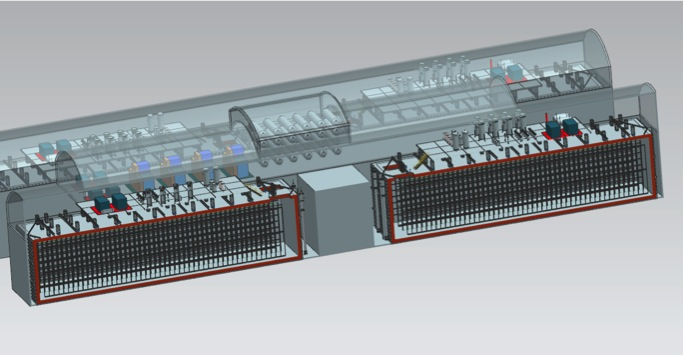
\includegraphics[width=.5\textwidth]{FarDet-3D-SP.jpg}
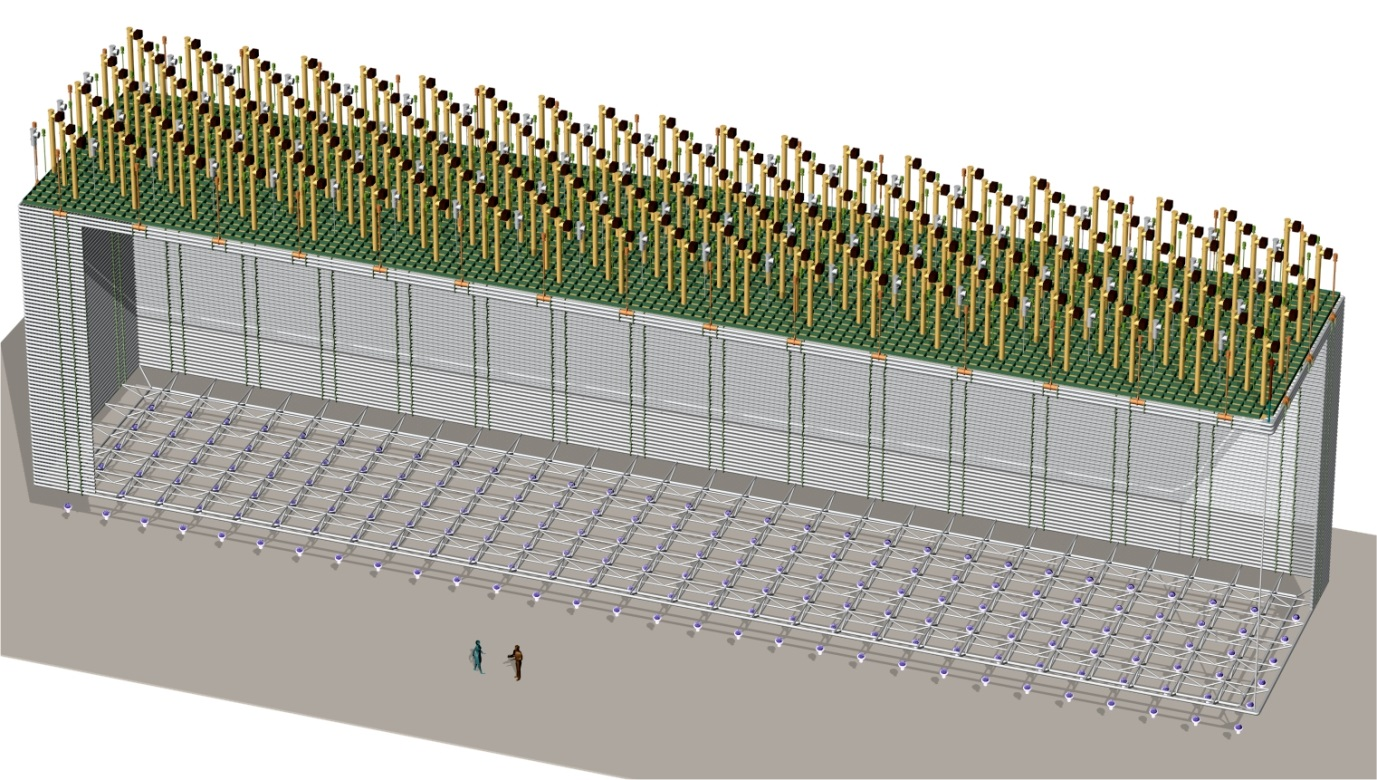
\includegraphics[width=0.46\textwidth]{DP_det2.jpg}
\end{center}
\end{minipage}
\end{cdrfigure}

Interactions in liquid argon (LAr) produce ionization charge and
scintillation light.  The electrons drift in a constant electric field
away from the cathode plane towards the segmented anode plane.  The
prompt scintillation light is observed by photodetectors that provide
the absolute time of the event.  The reference design, described in
Chapter~\ref{ch:detectors-fd-ref}, adopts a single-phase readout, in
which the readout anode is composed of wire planes in the LAr volume.
The alternate design, discussed in Chapter~\ref{ch:detectors-fd-alt},
considers the dual-phase approach, where ionization charge is
extracted, amplified and detected in gaseous argon above the liquid
surface.  The dual-phase design allows a finer readout pitch (3~mm), a
lower detection-energy threshold, and better pattern reconstruction of
the events.  Both the reference and alternate designs include systems
to collect the scintillation light.


A comprehensive prototyping strategy for both designs is being
actively pursued, as described in Chapter~\ref{ch:detectors-proto}.
The reference design, closer to the original ICARUS design, is
currently being validated in the 35-t prototype LAr detector at
Fermilab (see Section~\ref{sec:proto-35t}).  The novel alternative
design approach has been proven on several small-scale prototypes, and
a 20-t dual-phase prototype is being constructed at CERN, intended for
operation in 2016.  Full-scale engineering prototypes will be
assembled and commissioned at the CERN neutrino platform~\footnote{See
  CERN Bulletin article at
  \href{http://cds.cern.ch/journal/CERNBulletin/2014/51/News\%20Articles/1975980?ln=en}{http://cds.cern.ch/journal/CERNBulletin/2014/51/News\%20Articles/1975980?ln=en}.};
they are expected to provide the ultimate validation of the engineered
solutions for both far detector designs around the year 2018.

A test-beam data campaign will be executed in the following years to
collect a large sample of charged particle interactions to study the
detector response with high precision.

The deployment of the four 10-kt modules at SURF will take several
years and be guided by principles detailed in
Chapter~\ref{ch:detectors-strategy}. According to this strategy, DUNE
adopts the lowest-risk design that satisfies the physics and detector
requirements and allows installation of the first 10-kt detector
module as early as possible.  Accordingly, the first 10-kt module will
implement the reference design.  Installation of the second 10-kt
module will commence soon after the first one is implemented
\fixme{right? It used to say `soon thereafter' (Actually, I think we
  could get rid of this whole sentence. Anne)} and will be
instrumented as soon as possible.


A clear and transparent decision process will be adopted for
determining the design of the second and subsequent modules.  The
decision will be based on physics performance, technical and schedule
risks, costs and funding opportunities.  Besides taking advantage of
technological developments, a flexible approach to the far detector
design acknowledges the diversity of DUNE and offers the potential to
attract additional interest and resources into the Collaboration. A
staged approach provides access to an early science program while
allowing for new developments to be implemented over the relatively
long installation period of the experiment.

%%%%%%%%%%%%%%%%%%%%%%%%%%%%%%%
\subsection{Near Detector Systems}
\label{sec:intro-dune-near-det}

DUNE will install a near neutrino detector (NND) $\sim$0.5~km
downstream of the target and a Beamline Measurement System (BLM)
$\sim$300~m upstream of the NND. These are collectively called the
Near Detector Systems (NDS).  The NDS will allow DUNE to reduce
systematic errors to match the high-statistics phase precision sensitivity
for the long-baseline neutrino oscillation studies.  The primary role
of the neutrino detector is to measure the spectrum and flavor
composition of the beam to high precision. This detector will be
magnetized so that it can charge-discriminate electrons and muons
produced in the neutrino charged current interactions; it will
therefore be capable of making separate measurements of the neutrino
and antineutrino fluxes.
%
%In order to reach the ultimate
%sensitivity for the long-baseline neutrino oscillation studies, the neutrino detector will
%measure the spectrum and flavor composition of the (neutrino beam to high precision.  
%Separate measurements of the fluxes of neutrinos and antineutrinos requires a
%magnetized neutrino detector to charge-discriminate electrons and
%muons produced in the neutrino charged current interactions.  This is
%the primary role of the DUNE near detector; % system; 
%however, 

In addition, exposure to the intense neutrino flux provides the
opportunity to collect neutrino interaction data sets of unprecedented
size, enabling an extended science program.  The near detector
therefore provides an opportunity for a wealth of fundamental neutrino
interaction measurements, which are an important part of the ancillary
scientific goals of the DUNE collaboration.

The reference design for the neutrino near detector (NND) design is
the NOMAD-inspired fine-grained tracker (FGT) and is described in
Chapter~\ref{ch:detectors-nd-ref}. The NND subsystems include a
central straw-tube tracker and an electromagnetic calorimeter embedded
in a 0.4-T dipole field. The magnet yoke steel will be instrumented
with muon identifiers.

The Beamline Measurement System (BLM), designed to measure the muon
flux from hadron decay, is located in the region of the beam absorber
at the downstream end of the decay region. It is intended to monitor
the beam profile on a spill-by-spill basis and will operate for the
life of the experiment.
